\documentclass[11pt,a4paper]{article}
\usepackage[utf8]{inputenc}
\usepackage[T1]{polski}
\usepackage[margin=2.5cm]{geometry}
\usepackage{graphicx}
\usepackage{booktabs}
\usepackage{amsmath}
\usepackage{amssymb}
\usepackage{fancyhdr}
\usepackage{float}
\setlength{\headheight}{13.6pt}
\usepackage{hyperref}

% Konfiguracja nagłówka i stopki
\pagestyle{fancy}
\fancyhf{}
\fancyhead[L]{Algorytmy geometryczne — Ćwiczenie 1}
\fancyhead[R]{Elżbieta Łabaj}
\fancyfoot[C]{\thepage}

\begin{document}

% --- STRONA TYTUŁOWA / NAGŁÓWEK ---
\begin{center}
    {\LARGE \textbf{Sprawozdanie z ćwiczenia nr 1}} \\[0.5em]
    {\Large Predykaty geometryczne} \\[1.5em]
    
    \begin{tabular}{rl}
        \textbf{Autor:} & Elżbieta Łabaj \\
        \textbf{Data:} & \today \\
    \end{tabular}
\end{center}

\vspace{1em}
\hrule
\vspace{1em}

% ==========================================
\section{Dane techniczne}
% ==========================================
Specyfikacja środowiska obliczeniowego oraz parametrów technicznych:
\begin{itemize}
    \item \textbf{Język programowania:} Python 3.13.13
    \item \textbf{Procesor:} Intel(R) Core(TM) i5-8265U CPU 1.60GHz

    \item \textbf{System operacyjny:} Fedora Linux (x86\char`_64)
\end{itemize}

% ==========================================
\section{Realizacja ćwiczenia}
% ==========================================
\subsection{Generowanie zbiorów punktów:}
    
    Wygenerowano następujące zbiory punktów używając \texttt{np.random.uniform}:
    \begin{itemize}
        \item \textbf{Zbiór a:} $10^5$ losowych punktów z przedziału $[-1000, 1000] \times [-1000, 1000]$.
        \item \textbf{Zbiór b:} $10^5$ losowych punktów z przedziału $[-10^{14}, 10^{14}] \times [-10^{14}, 10^{14}]$.
        \item \textbf{Zbiór c:} 1000 punktów na okręgu o środku $(0,0)$ i promieniu $r=100$, wygenerowanych z równania parametrycznego ($x = r \cos(2 \pi t)$, $y = r \sin(2 \pi t)$, $t \in [0, 1]$).
        \item \textbf{Zbiór d:} 1000 punktów leżących na prostej wyznaczonej przez wektor $AB$, gdzie $A = (-1.0, 0.0)$ oraz $B = (1.0, 0.1)$.
    \end{itemize}

\begin{figure}[htbp]
    \centering
    \begin{minipage}{0.48\textwidth}
        \centering
        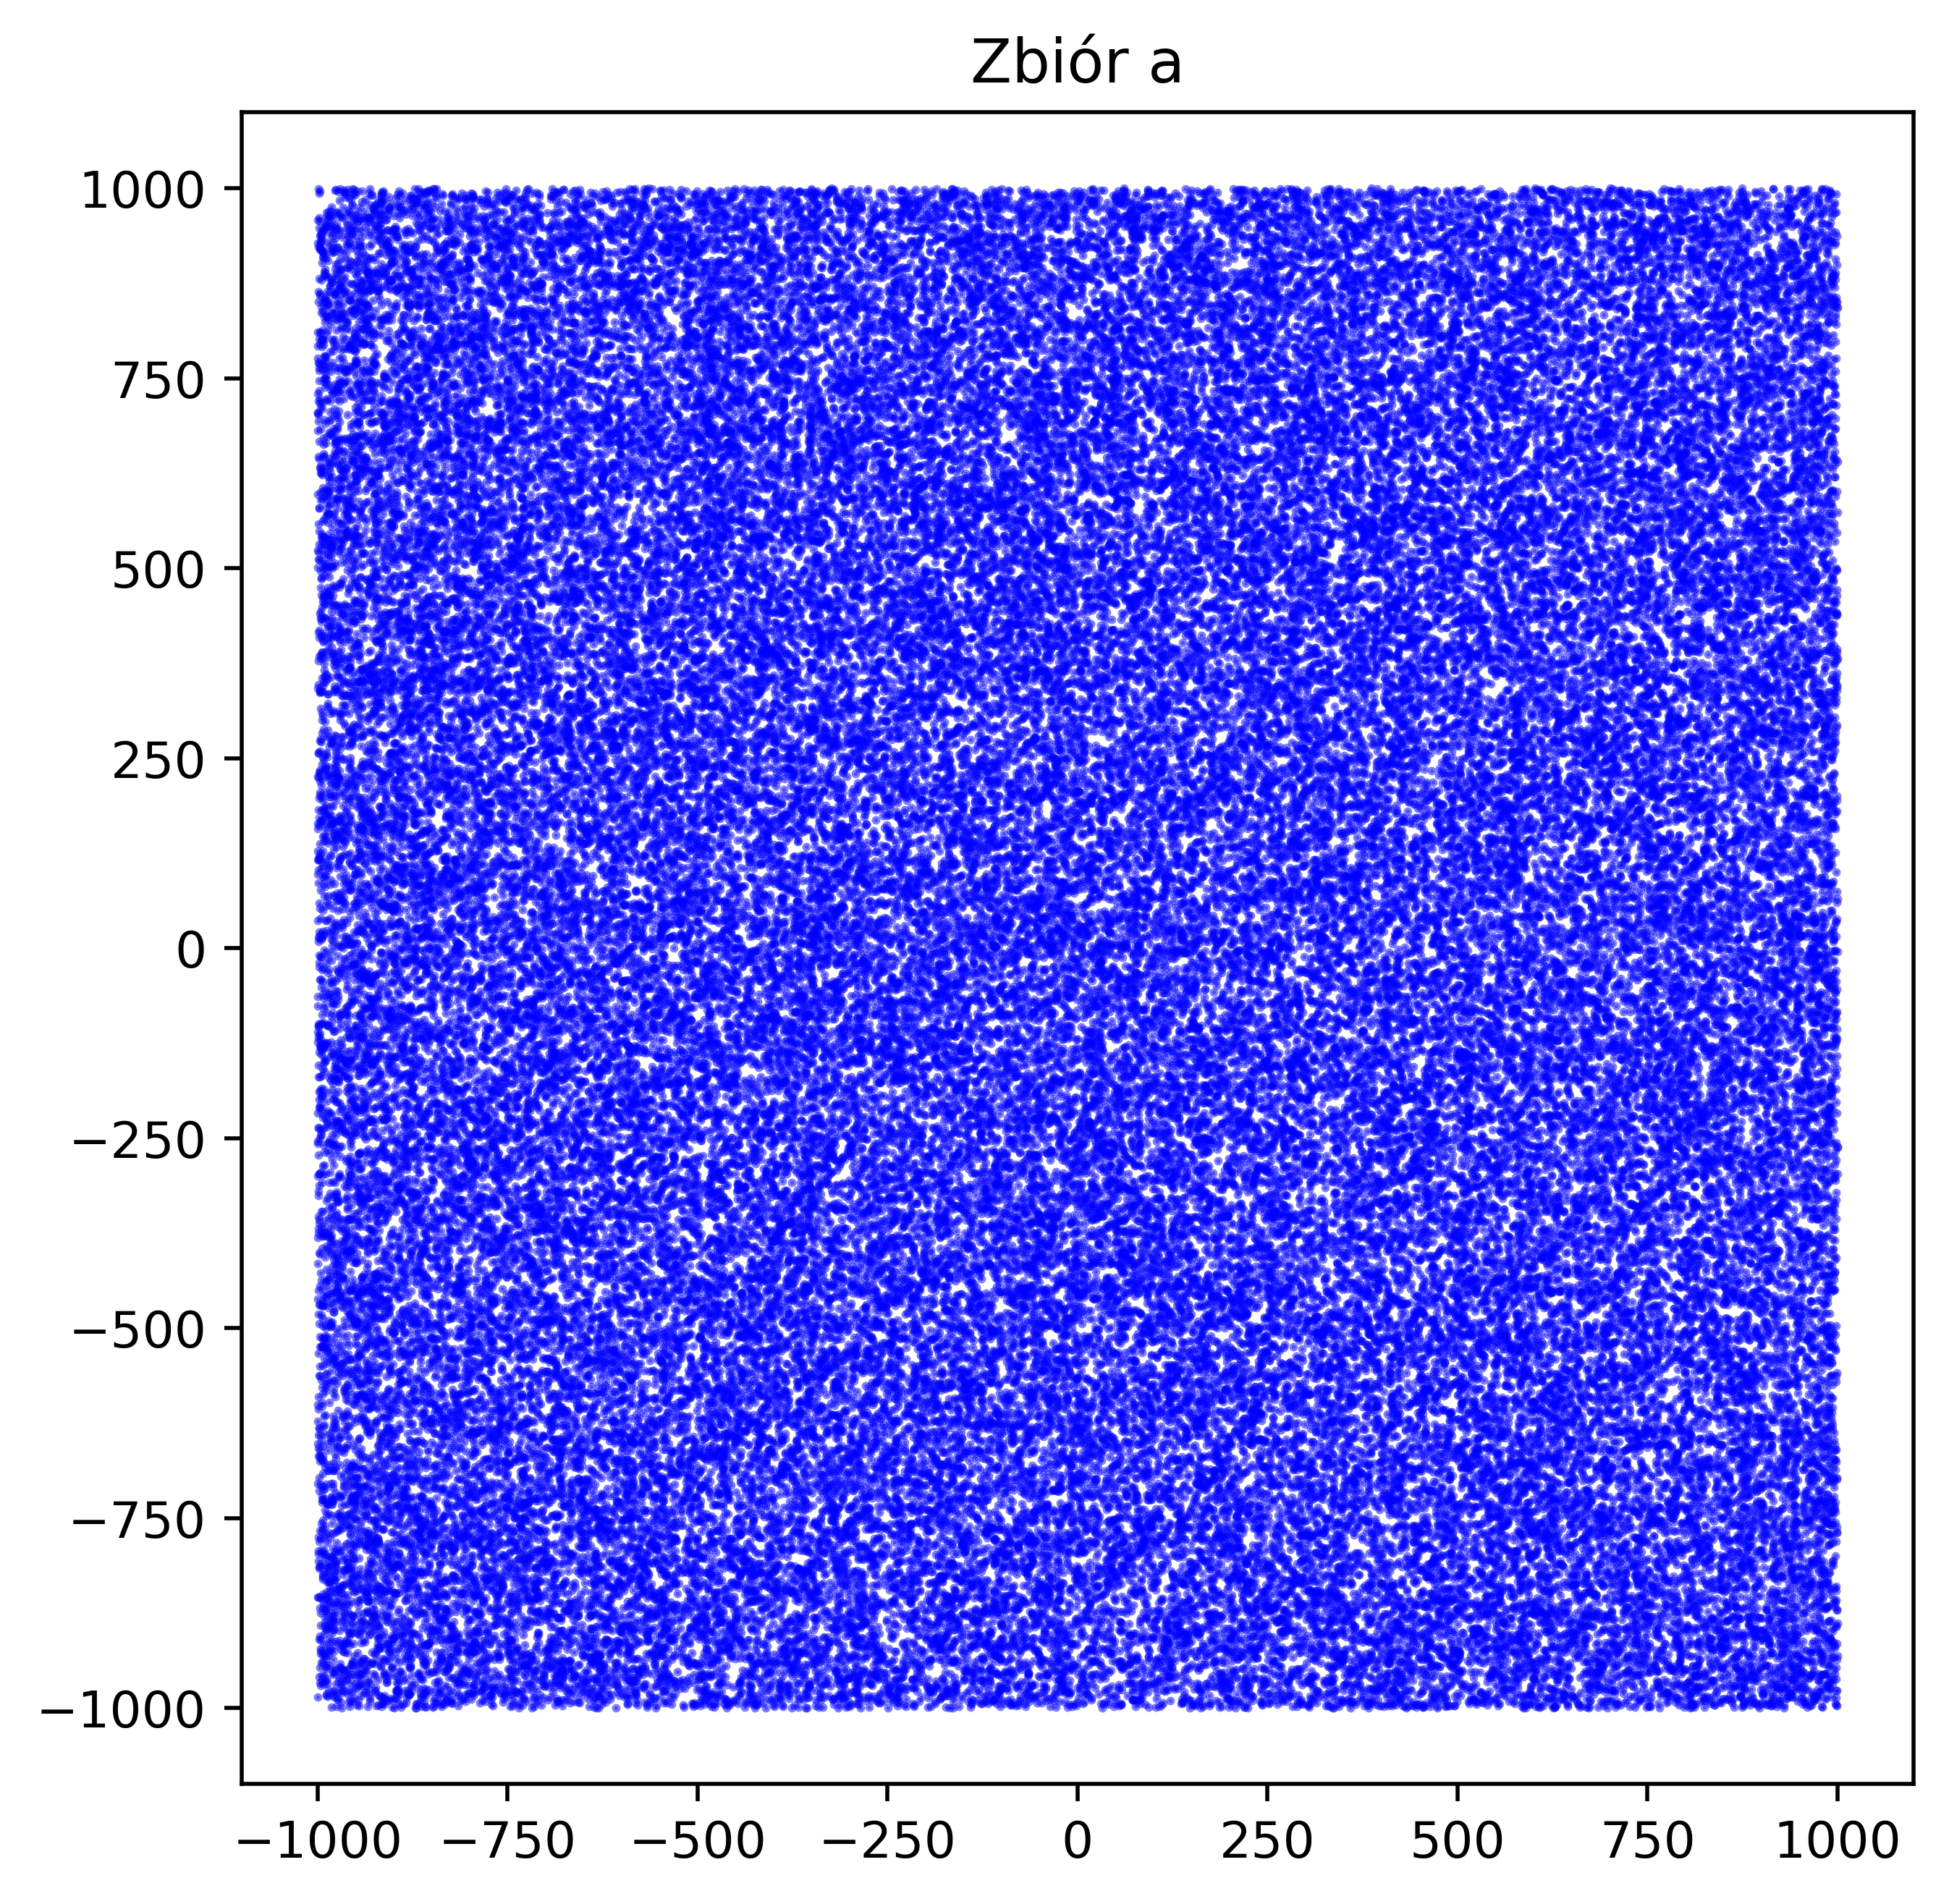
\includegraphics[width=\linewidth]{plots/dataset_a_raw.png}
        \caption{Zbiór a.}
        \label{fig:raw_a}
    \end{minipage}
    \hfill
    \begin{minipage}{0.48\textwidth}
        \centering
        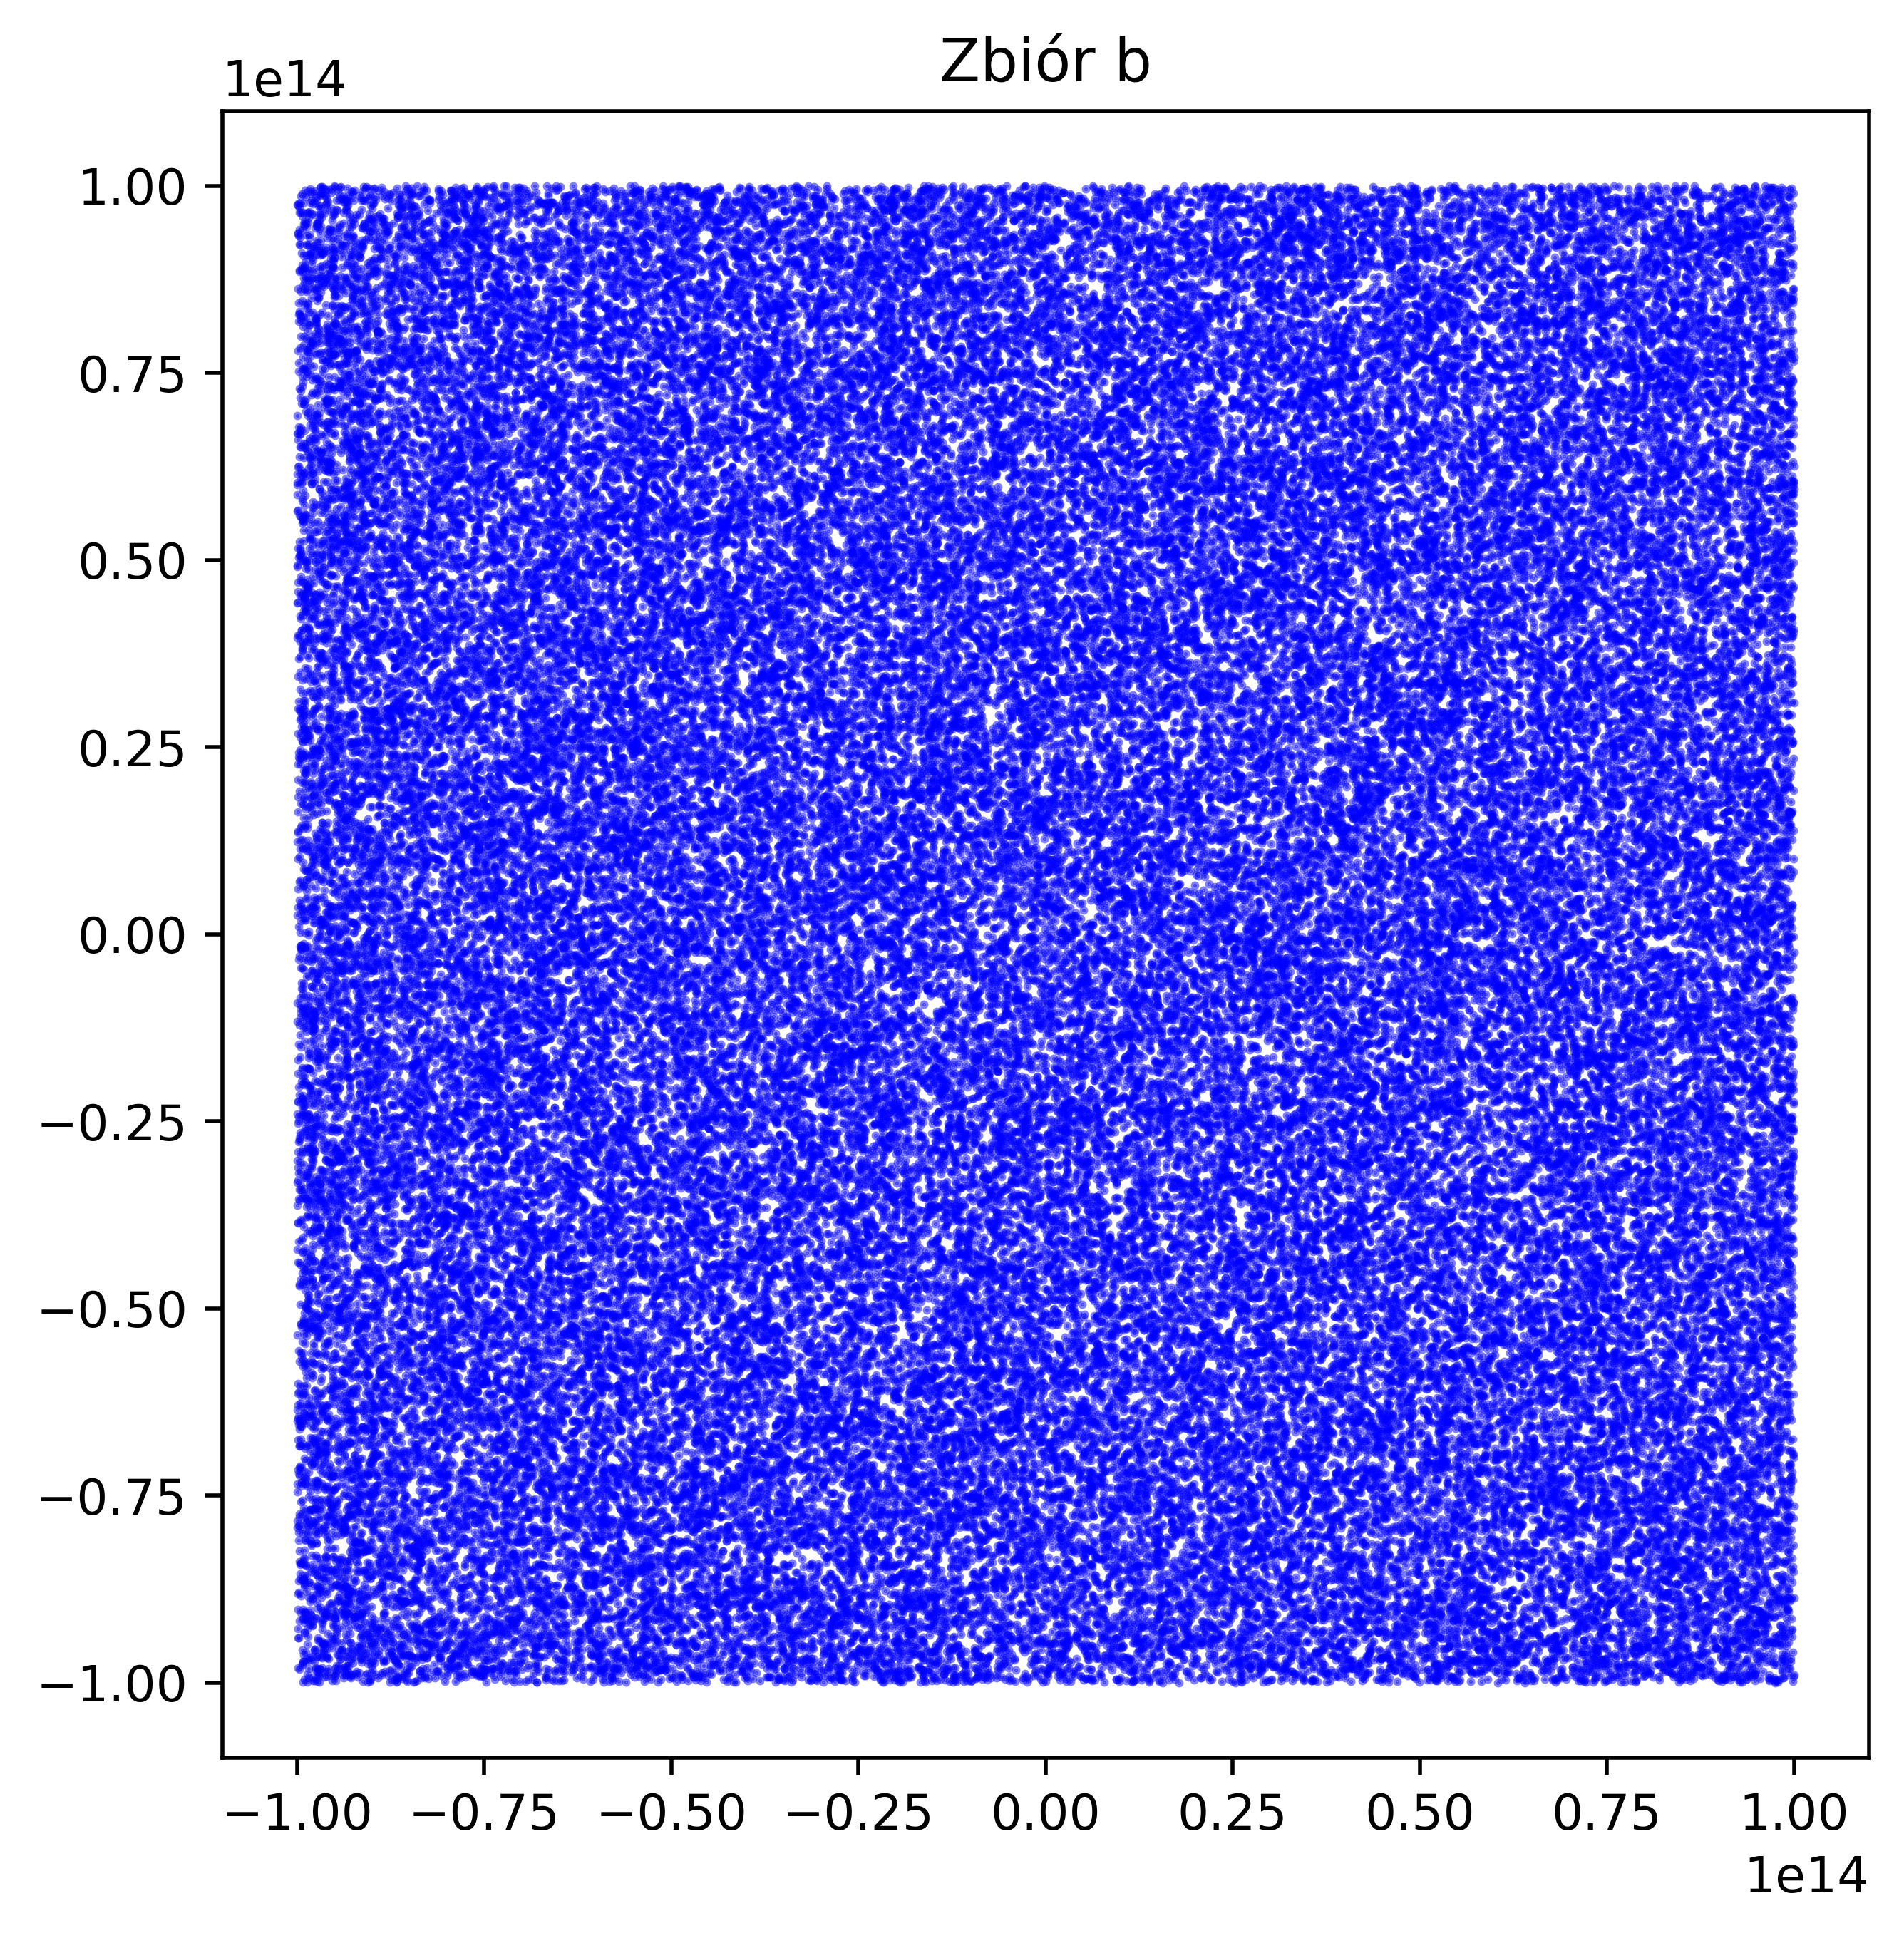
\includegraphics[width=\linewidth]{plots/dataset_b_raw.png}
        \caption{Zbiór b.}
        \label{fig:raw_b}
    \end{minipage}
\end{figure}

\clearpage

% --- Druga para wykresów (zbiory c i d) ---
\begin{figure}[htbp]
    \centering
    \begin{minipage}{0.48\textwidth}
        \centering
        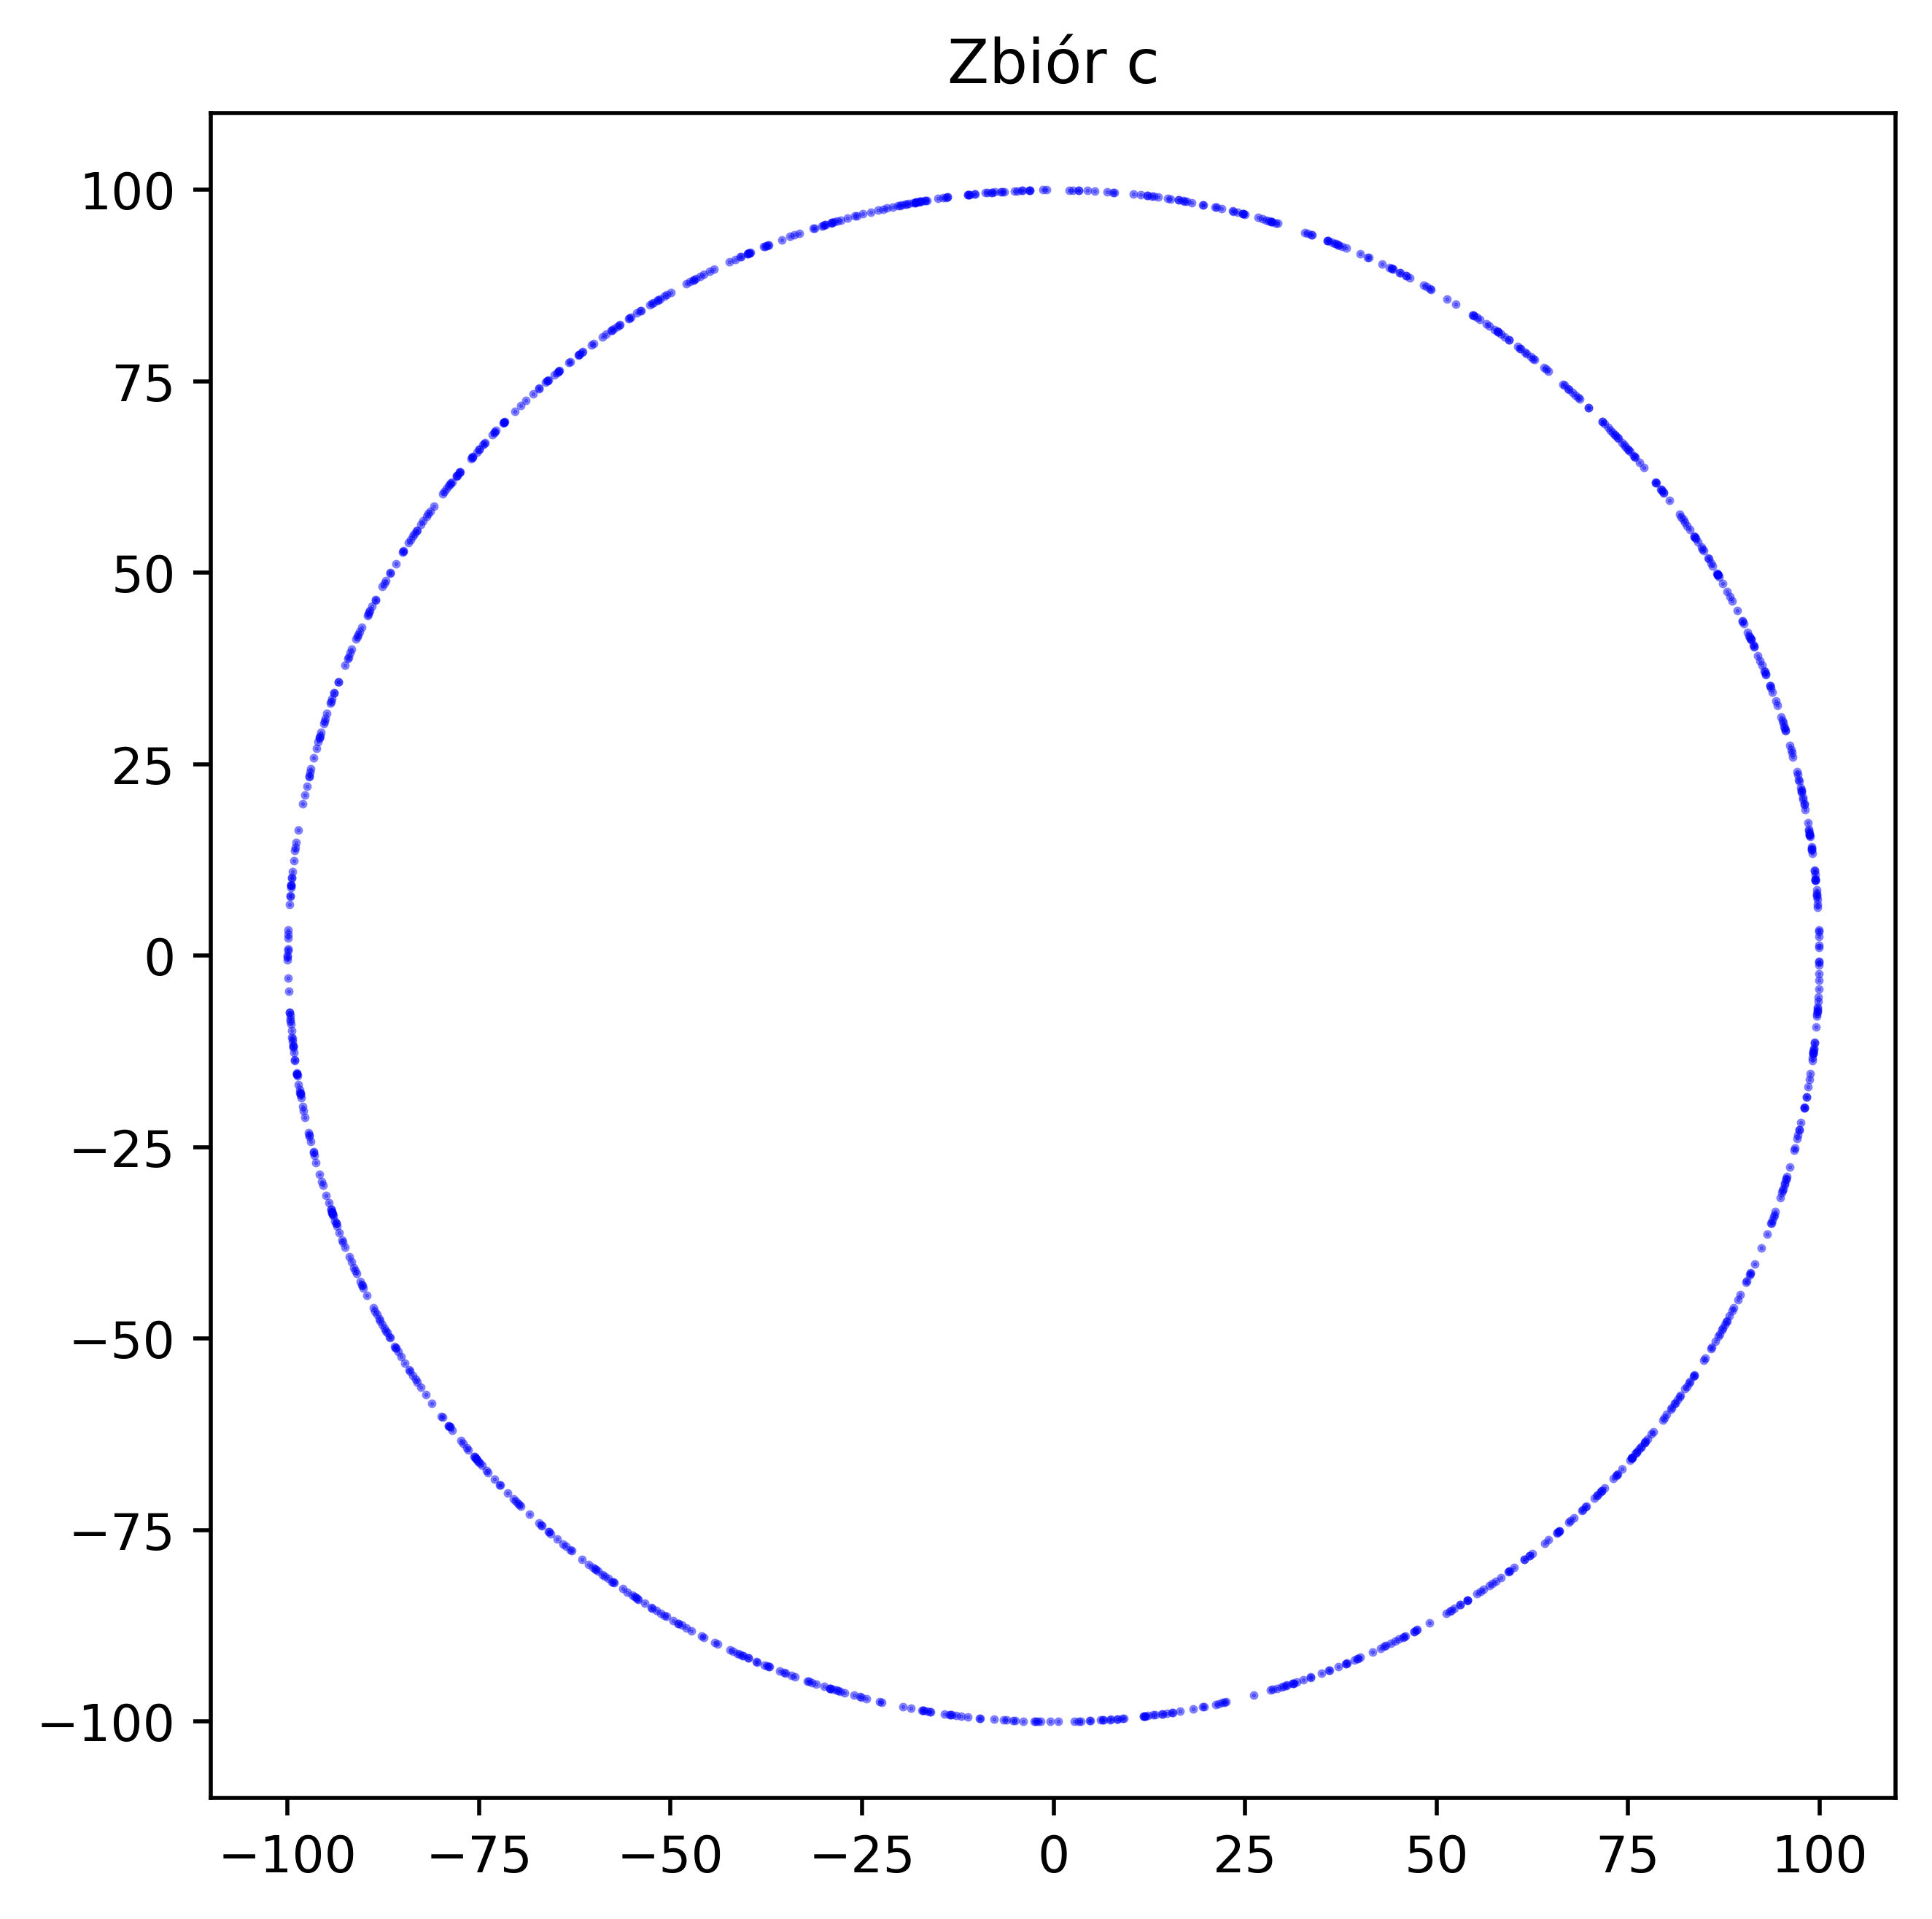
\includegraphics[width=\linewidth]{plots/dataset_c_raw.png}
        \caption{Zbiór c.}
        \label{fig:raw_c}
    \end{minipage}
    \hfill
    \begin{minipage}{0.48\textwidth}
        \centering
        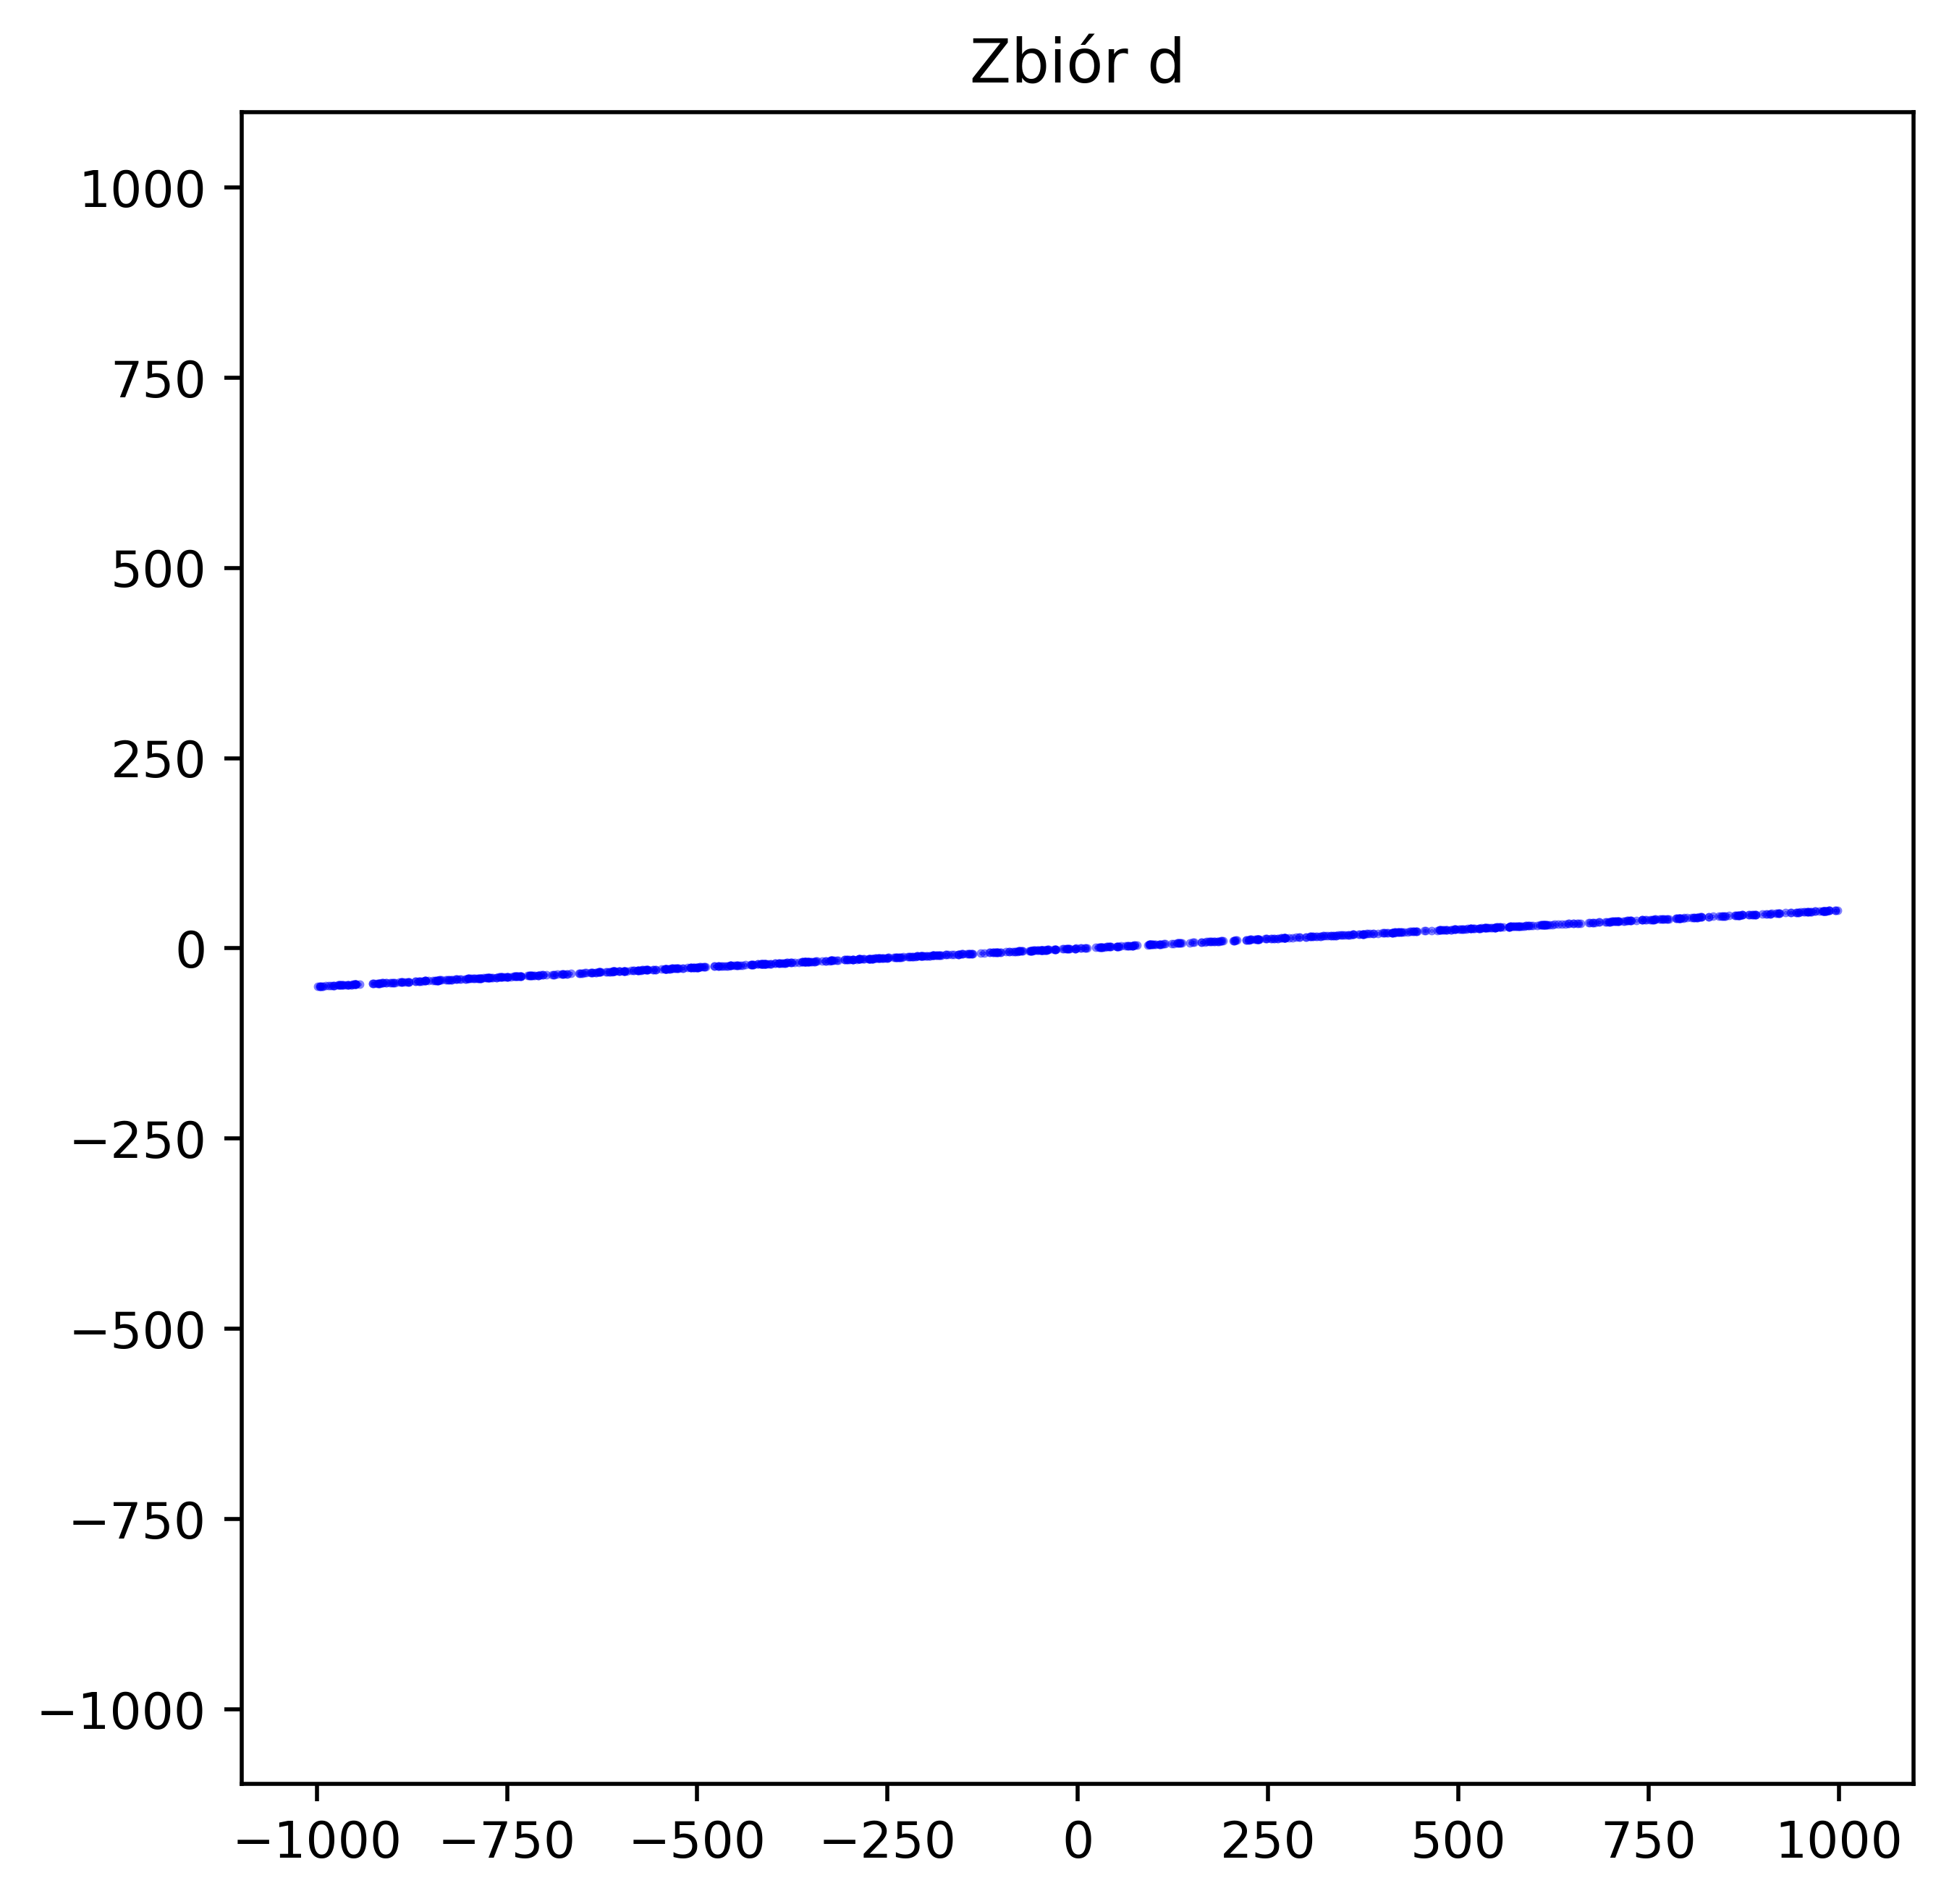
\includegraphics[width=\linewidth]{plots/dataset_d_raw.png}
        \caption{Zbiór d.}
        \label{fig:raw_d}
    \end{minipage}
\end{figure}

\subsection{Klasyfikacja punktów względem prostej:}
    
    Każdy punkt $c$ przydzielono do jednej z trzech kategorii względem prostej wyznaczanej przez wektor $ab$, gdzie $a = (-1.0, 0.0)$ oraz $b = (1.0, 0.1)$:
    \begin{itemize}
        \item na lewo od prostej (det $> \epsilon$),
        \item na prawo od prostej (det $< -\epsilon$),
        \item na prostej ($|$det$| < \epsilon$). 
    \end{itemize}
    Wyznacznik det liczono na cztery sposoby:
    \begin{enumerate}
    \item Wyznacznik macierzy ($3 \times 3$). Użyto metody własnej (\texttt{cross3x3})
    oraz \texttt{np.linalg.det} z biblioteki NumPy (\texttt{cross3x3\char`_numpy}).
    \begin{equation}
        \det(a, b, c) = \begin{vmatrix}
            a_x & a_y & 1 \\
            b_x & b_y & 1 \\
            c_x & c_y & 1
        \end{vmatrix}
    \end{equation}

    \item Wyznacznik macierzy ($2 \times 2$). Użyto metody własnej (\texttt{cross2x2})
    oraz \texttt{np.linalg.det} z biblioteki NumPy (\texttt{cross2x2\char`_numpy}).
    \begin{equation}
        \det(a, b, c) = \begin{vmatrix}
            a_x - c_x & a_y - c_y \\
            b_x - c_x & b_y - c_y
        \end{vmatrix}
    \end{equation}
    \end{enumerate}

    Użyto następujących wartości tolerancji dla zera ($\epsilon$): $10^{-6},10^{-9}, 10^{-12}$ oraz następujących typów danych: \texttt{float32}, \texttt{float64}.

\subsection{Analiza}

Analizowano poprawność oraz czas klasyfikacji punktów przez różne metody oraz dla różnych tolerancji i typów danych.

\clearpage

% ==========================================
\section{Wyniki}
% ==========================================

\subsection{Zbiory a i c}

Punkty w zbiorach a i c są równomiernie rozłożone, a ich współrzędne są z niewielkiego przedziału, dlatego dla obydwu zbiorów wszystkie metody sklasyfikowały wszystkie punkty poprawnie: $50242$ punkty po lewej stronie, $49758$ po prawej i $0$ punktów na prostej.

Metody z biblioteki były wolniejsze od metod własnych, a liczenie wyznaczników $3 \times 3$ było wolniejsze od $2 \times 2$. Dokladne zestawienie pokazano w Tabeli \ref{tab:wyniki_ac_12_minimal}.

\begin{figure}[htbp]
    \centering
    \begin{minipage}{0.48\textwidth}
        \centering
        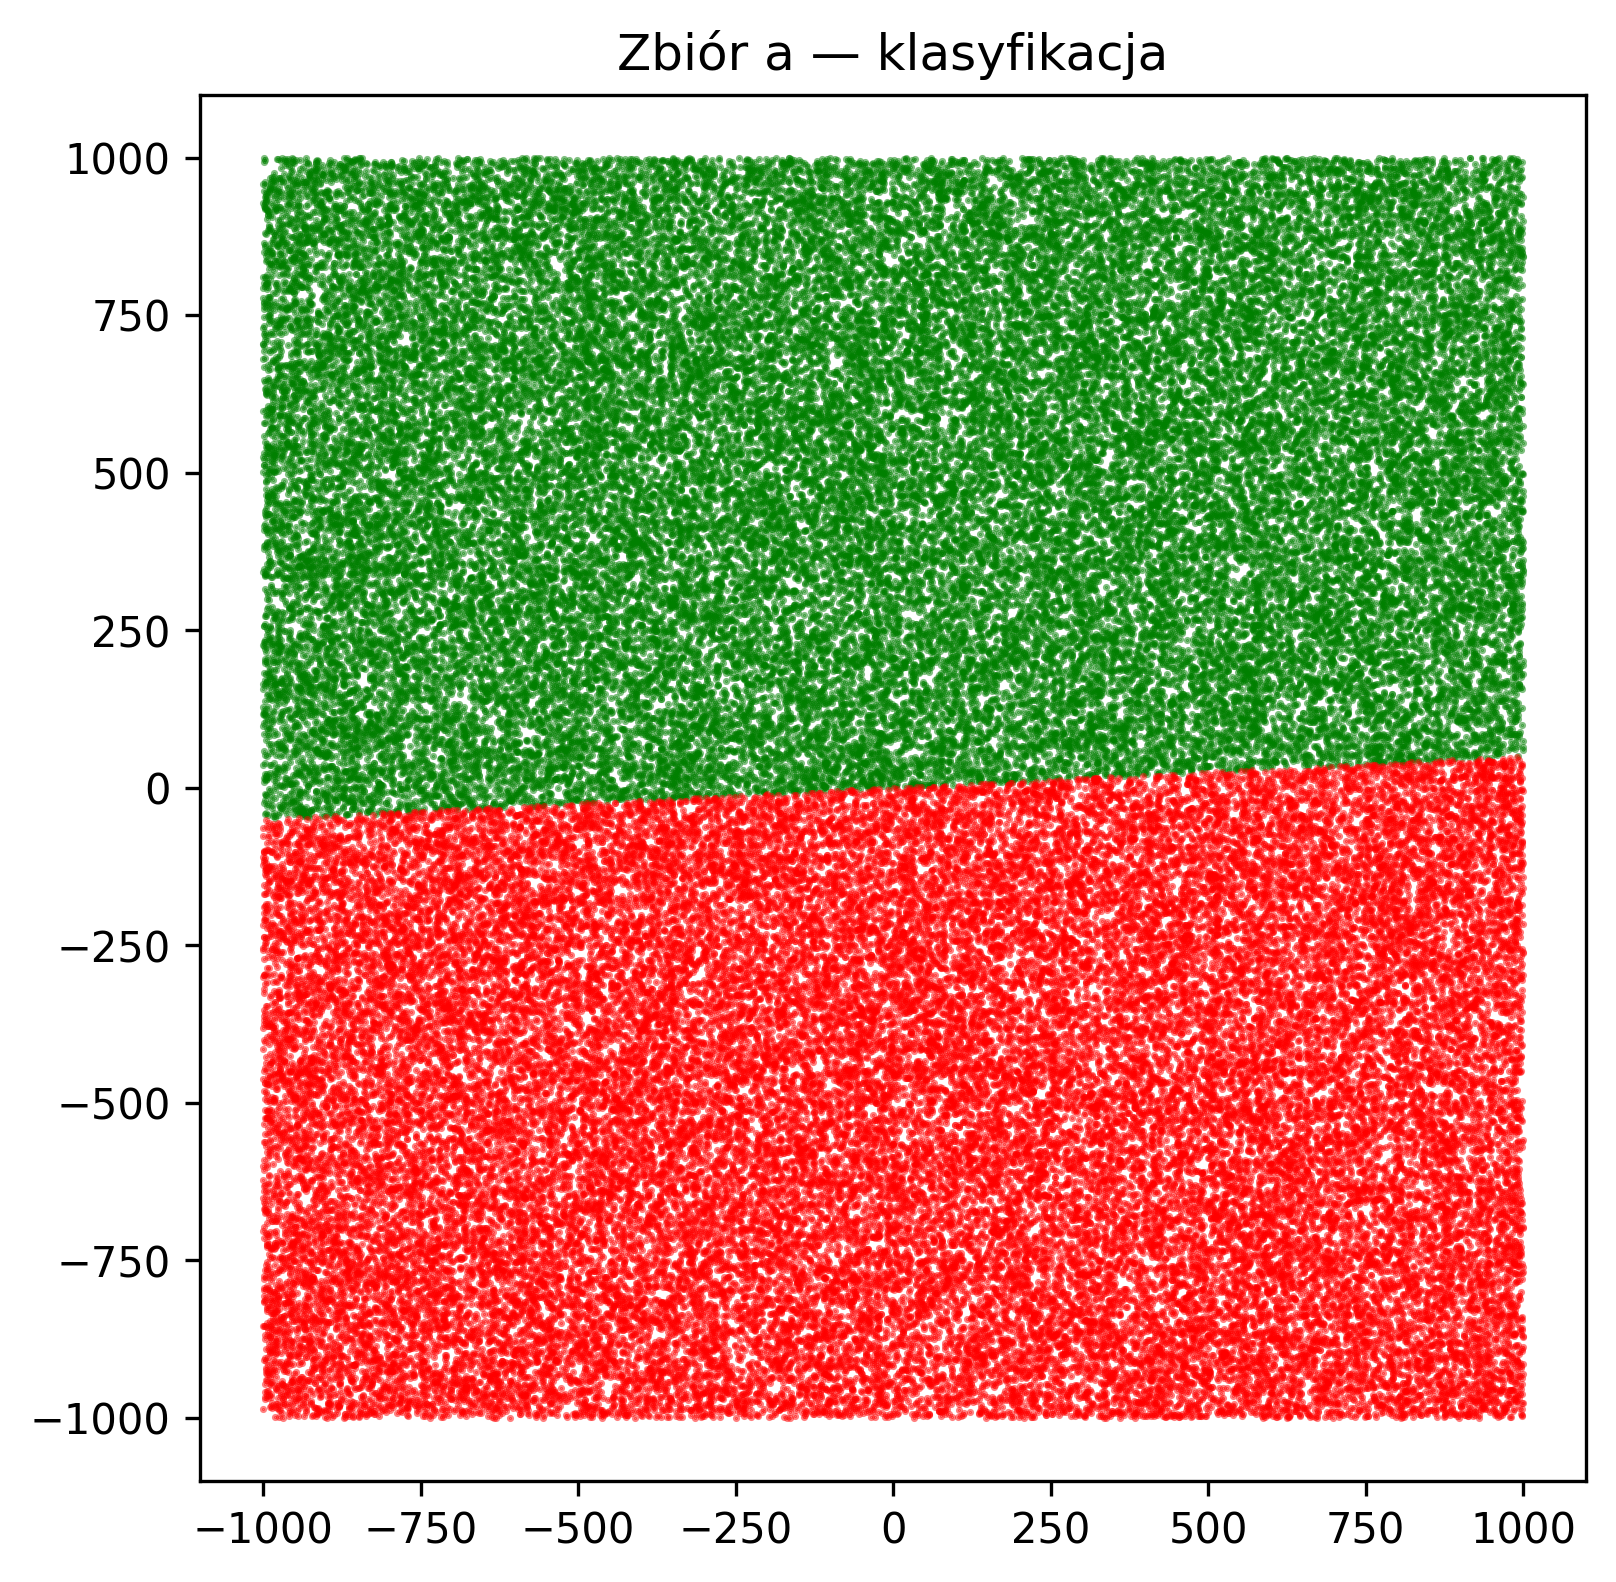
\includegraphics[width=\linewidth]{plots/dataset_a_classified.png}
        \caption{Klasyfikacja punktów ze zbioru a.}
        \label{fig:classified_a}
    \end{minipage}
    \hfill
    \begin{minipage}{0.48\textwidth}
        \centering
        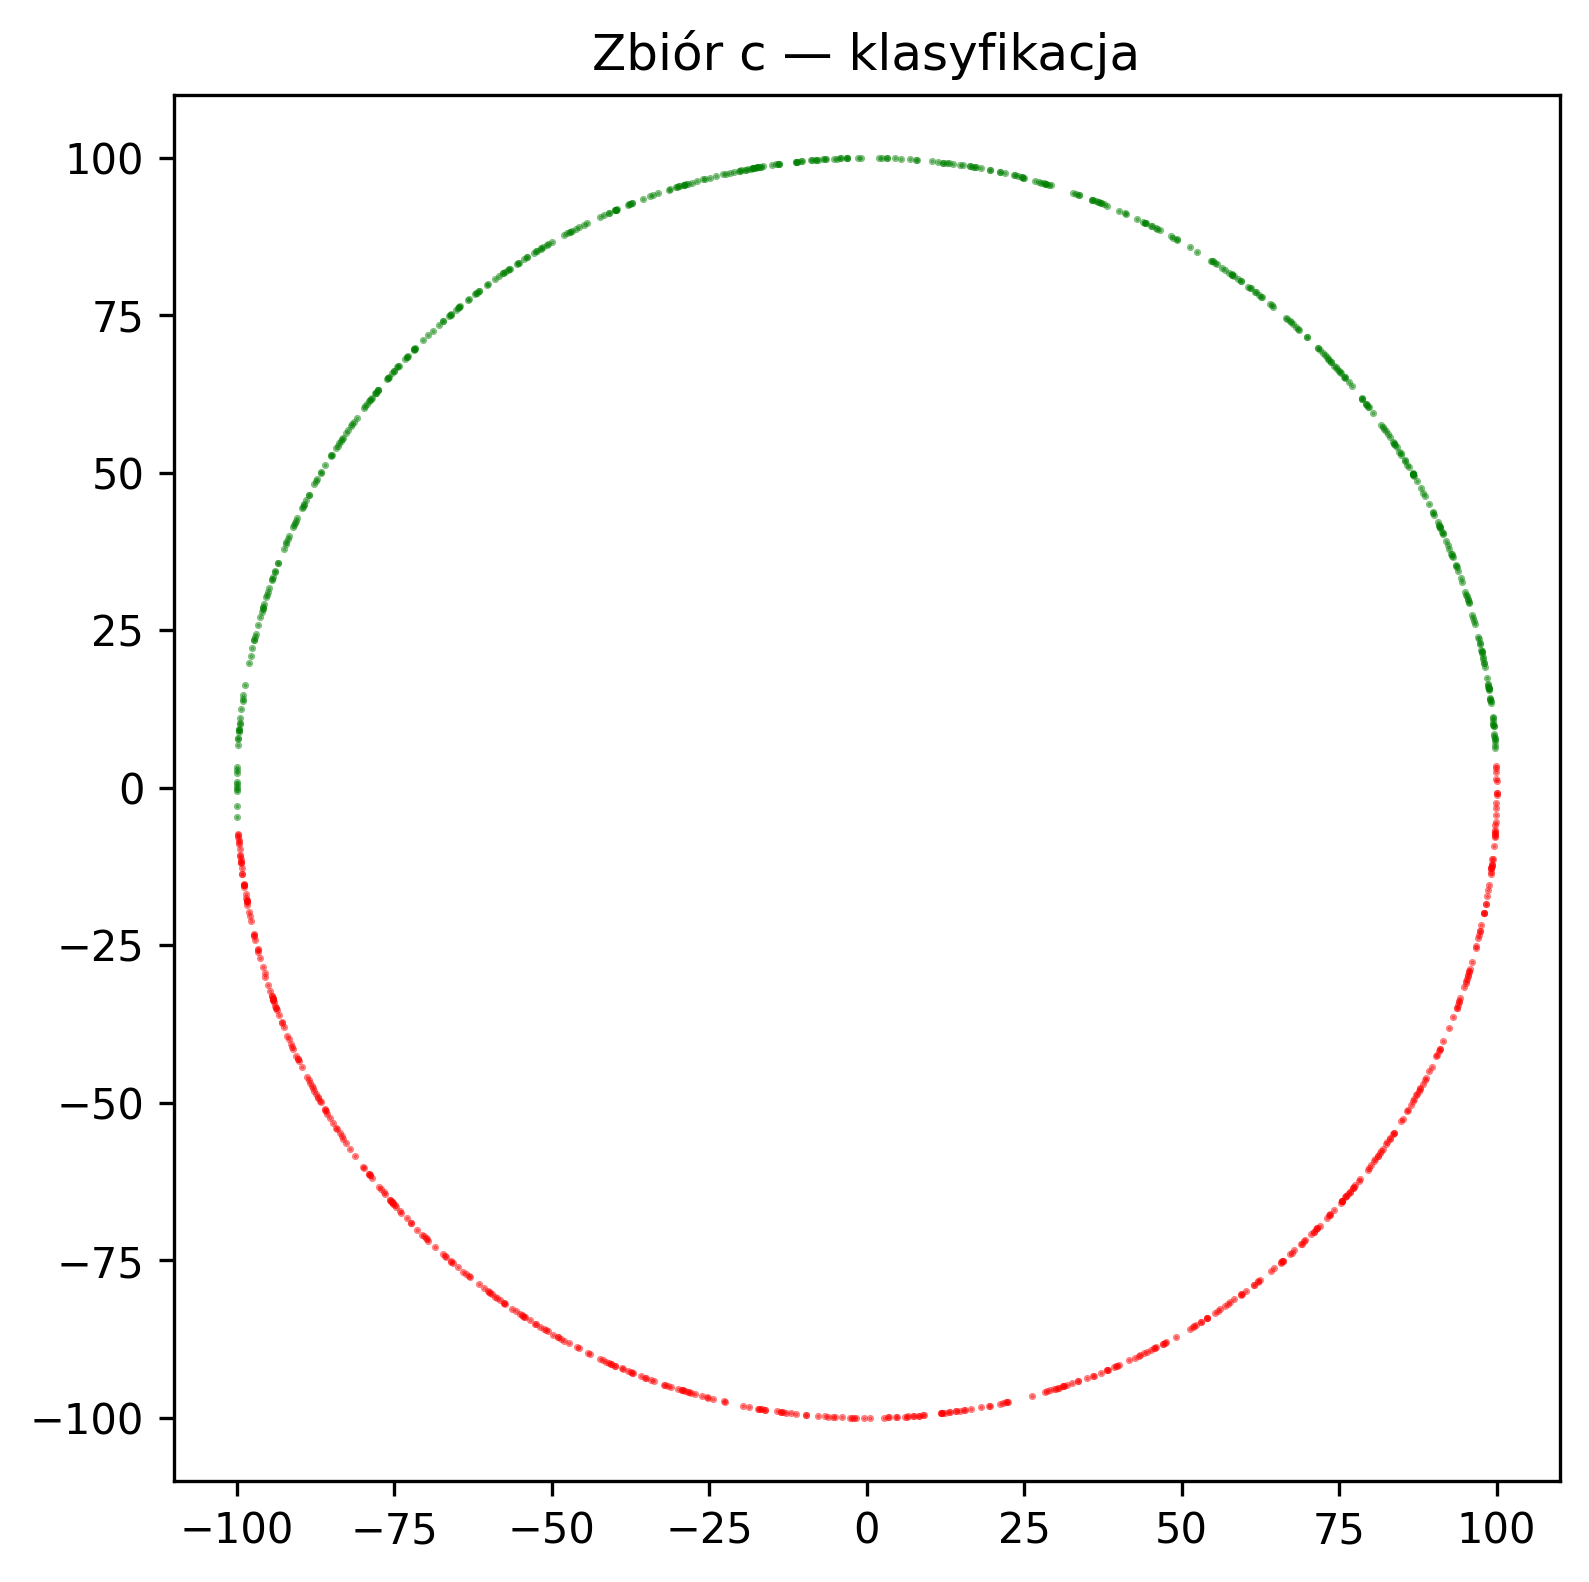
\includegraphics[width=\linewidth]{plots/dataset_c_classified.png}
        \caption{Klasyfikacja punktów ze zbioru c.}
        \label{fig:classified_c}
    \end{minipage}
\end{figure}

\begin{table}[htbp]
    \centering
    \caption{Zestawienie czasów wykonania metod dla zbiorów a i c.}
    \label{tab:wyniki_ac_12_minimal}
    \begin{tabular}{lllll}
        \toprule
        Zbiór & Typ danych & Epsilon & Metoda & Czas [s] \\
        \midrule
        a & \texttt{float64} & $10^{-12}$ & \texttt{3x3}        & 0.0056 \\
        a & \texttt{float64} & $10^{-12}$ & \texttt{2x2}        & 0.0049 \\
        a & \texttt{float64} & $10^{-12}$ & \texttt{3x3\_numpy} & 0.0295 \\
        a & \texttt{float64} & $10^{-12}$ & \texttt{2x2\_numpy} & 0.0192 \\
        \midrule
        c & \texttt{float64} & $10^{-12}$ & \texttt{3x3}        & 0.0001 \\
        c & \texttt{float64} & $10^{-12}$ & \texttt{2x2}        & 0.0000 \\
        c & \texttt{float64} & $10^{-12}$ & \texttt{3x3\_numpy} & 0.0003 \\
        c & \texttt{float64} & $10^{-12}$ & \texttt{2x2\_numpy} & 0.0002 \\
        \bottomrule
    \end{tabular}
\end{table}

\subsection{Zbiór b}

W zbiorze b współrzędne punktów były rzędu $10^{14}$ co spowodowało ogromny błąd przy klasyfikacji metodą wyznaczników macierzy $2 \times 2$. W tej metodzie liczone są najpierw różnice współrzędnych co zwłaszcza przy niskiej precyzji typu \texttt{float32} prowadzi do dużych błędów zaokrągleń i do fałszywej klasyfikacji punków jako współliniowych. 

Na Rysunku \ref{fig:classified_b_64} pokazano rozkład punktów przy użyciu typu \texttt{float64} oraz metody \texttt{cross2x2\_numpy}, a na Rysunku \ref{fig:classified_b_32} ten sam rozkład, ale przy użyciu typu \texttt{float32}. Na czarno zaznaczono punkty uznane za leżące na prostej. 

W Tabeli \ref{tab:wyniki_b_all_eps} pokazano wyniki klasyfikacji również dla reszty metod.
Wybór epsilona (tolerancji dla zera) nie wpływał na poprawność żadnej z metod.

\begin{figure}[htbp]
    \centering
    \begin{minipage}{0.48\textwidth}
        \centering
        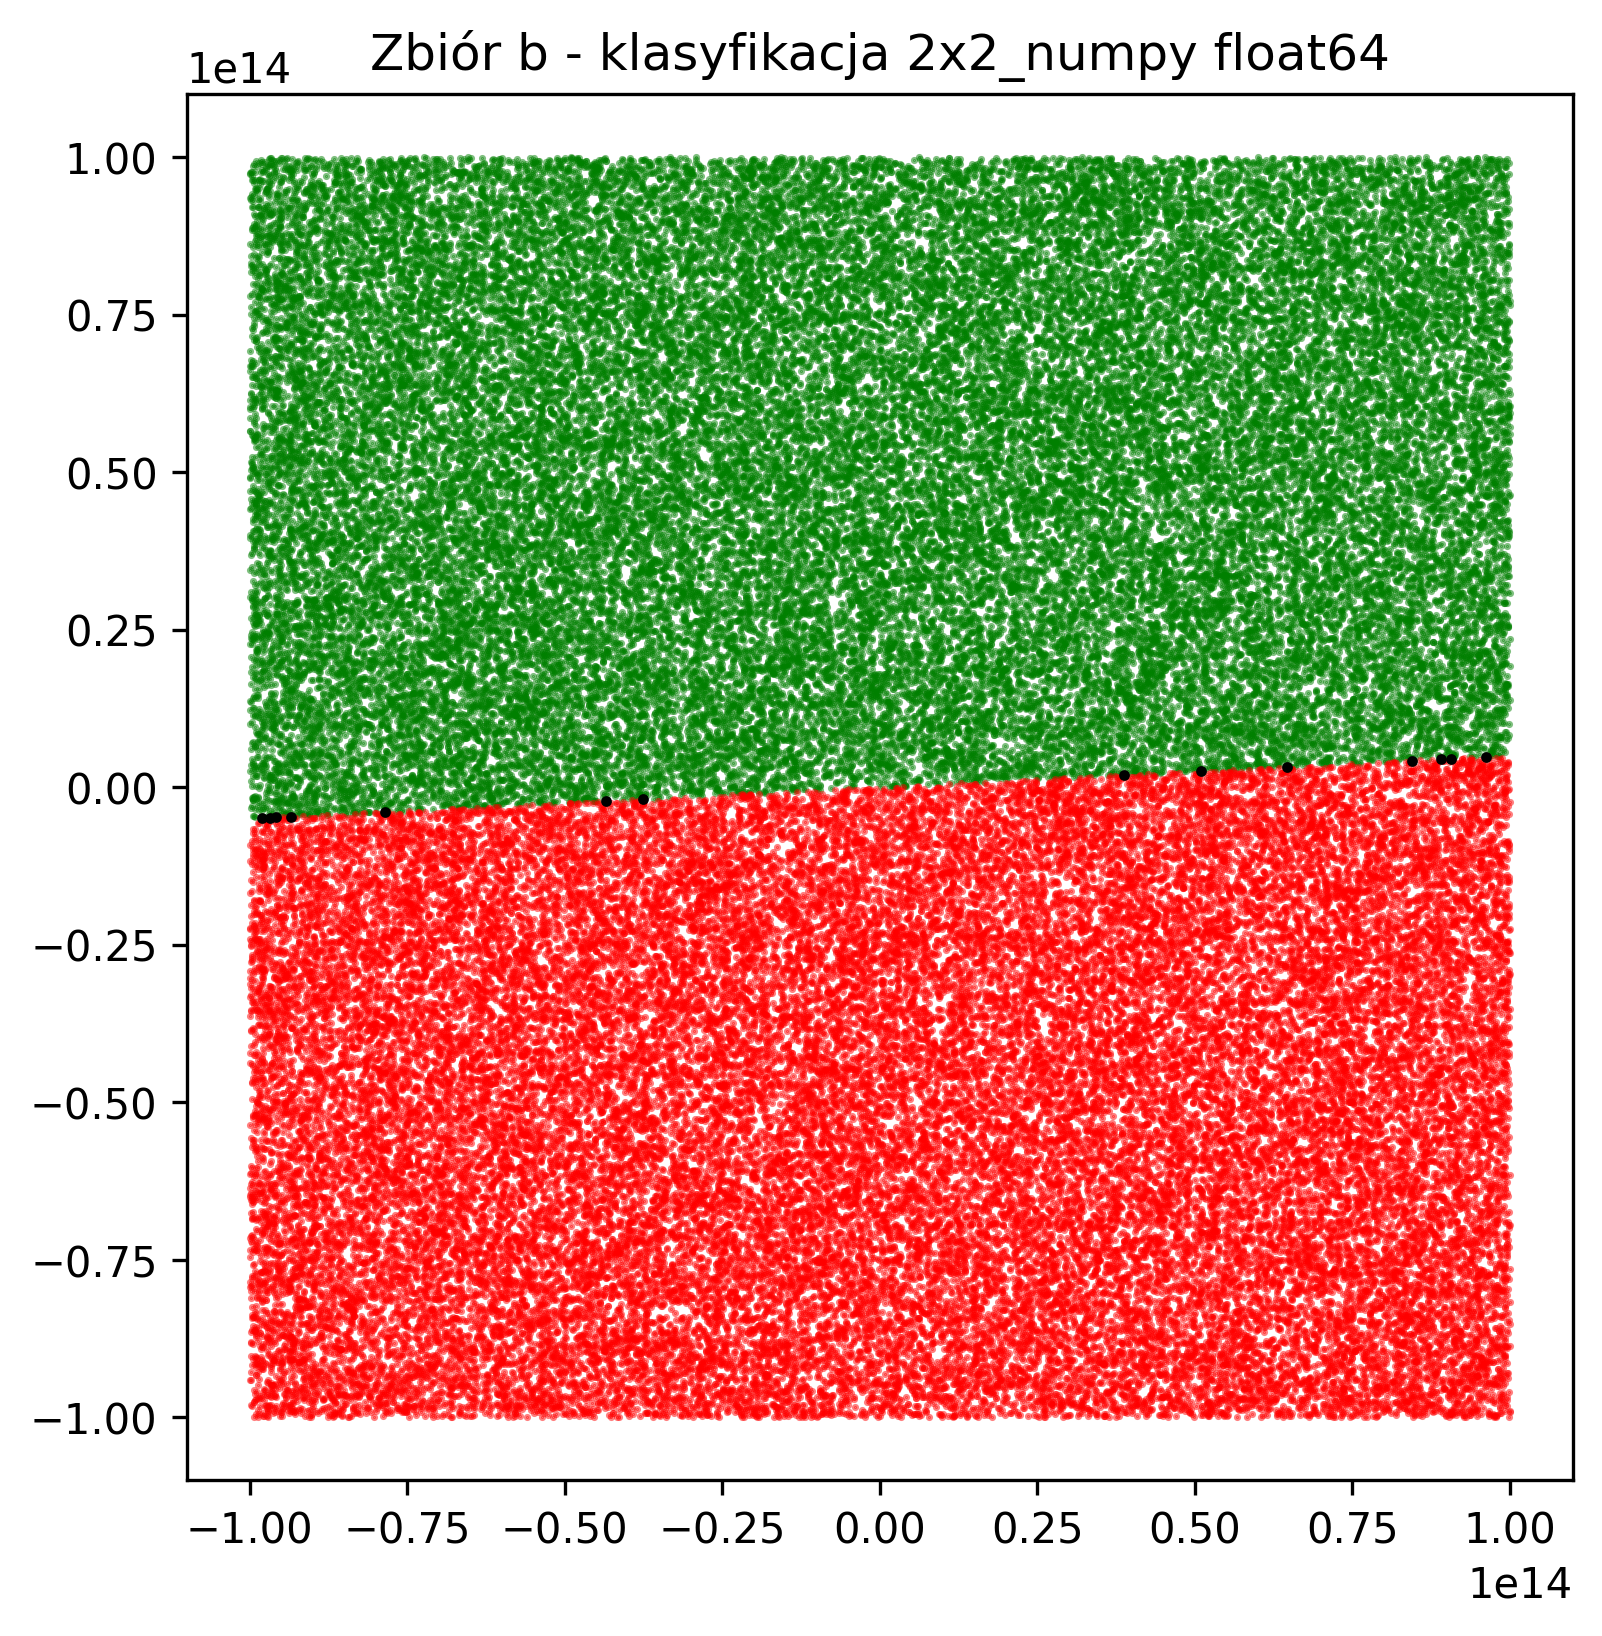
\includegraphics[width=\linewidth]{plots/dataset_Zbiór b - klasyfikacja 2x2_numpy float64_1e-06.png}
        \caption{Klasyfikacja punktów ze zbioru b metodą \texttt{2x2\_numpy} na typie \texttt{float64}.}
        \label{fig:classified_b_64}
    \end{minipage}
    \hfill
    \begin{minipage}{0.48\textwidth}
        \centering
        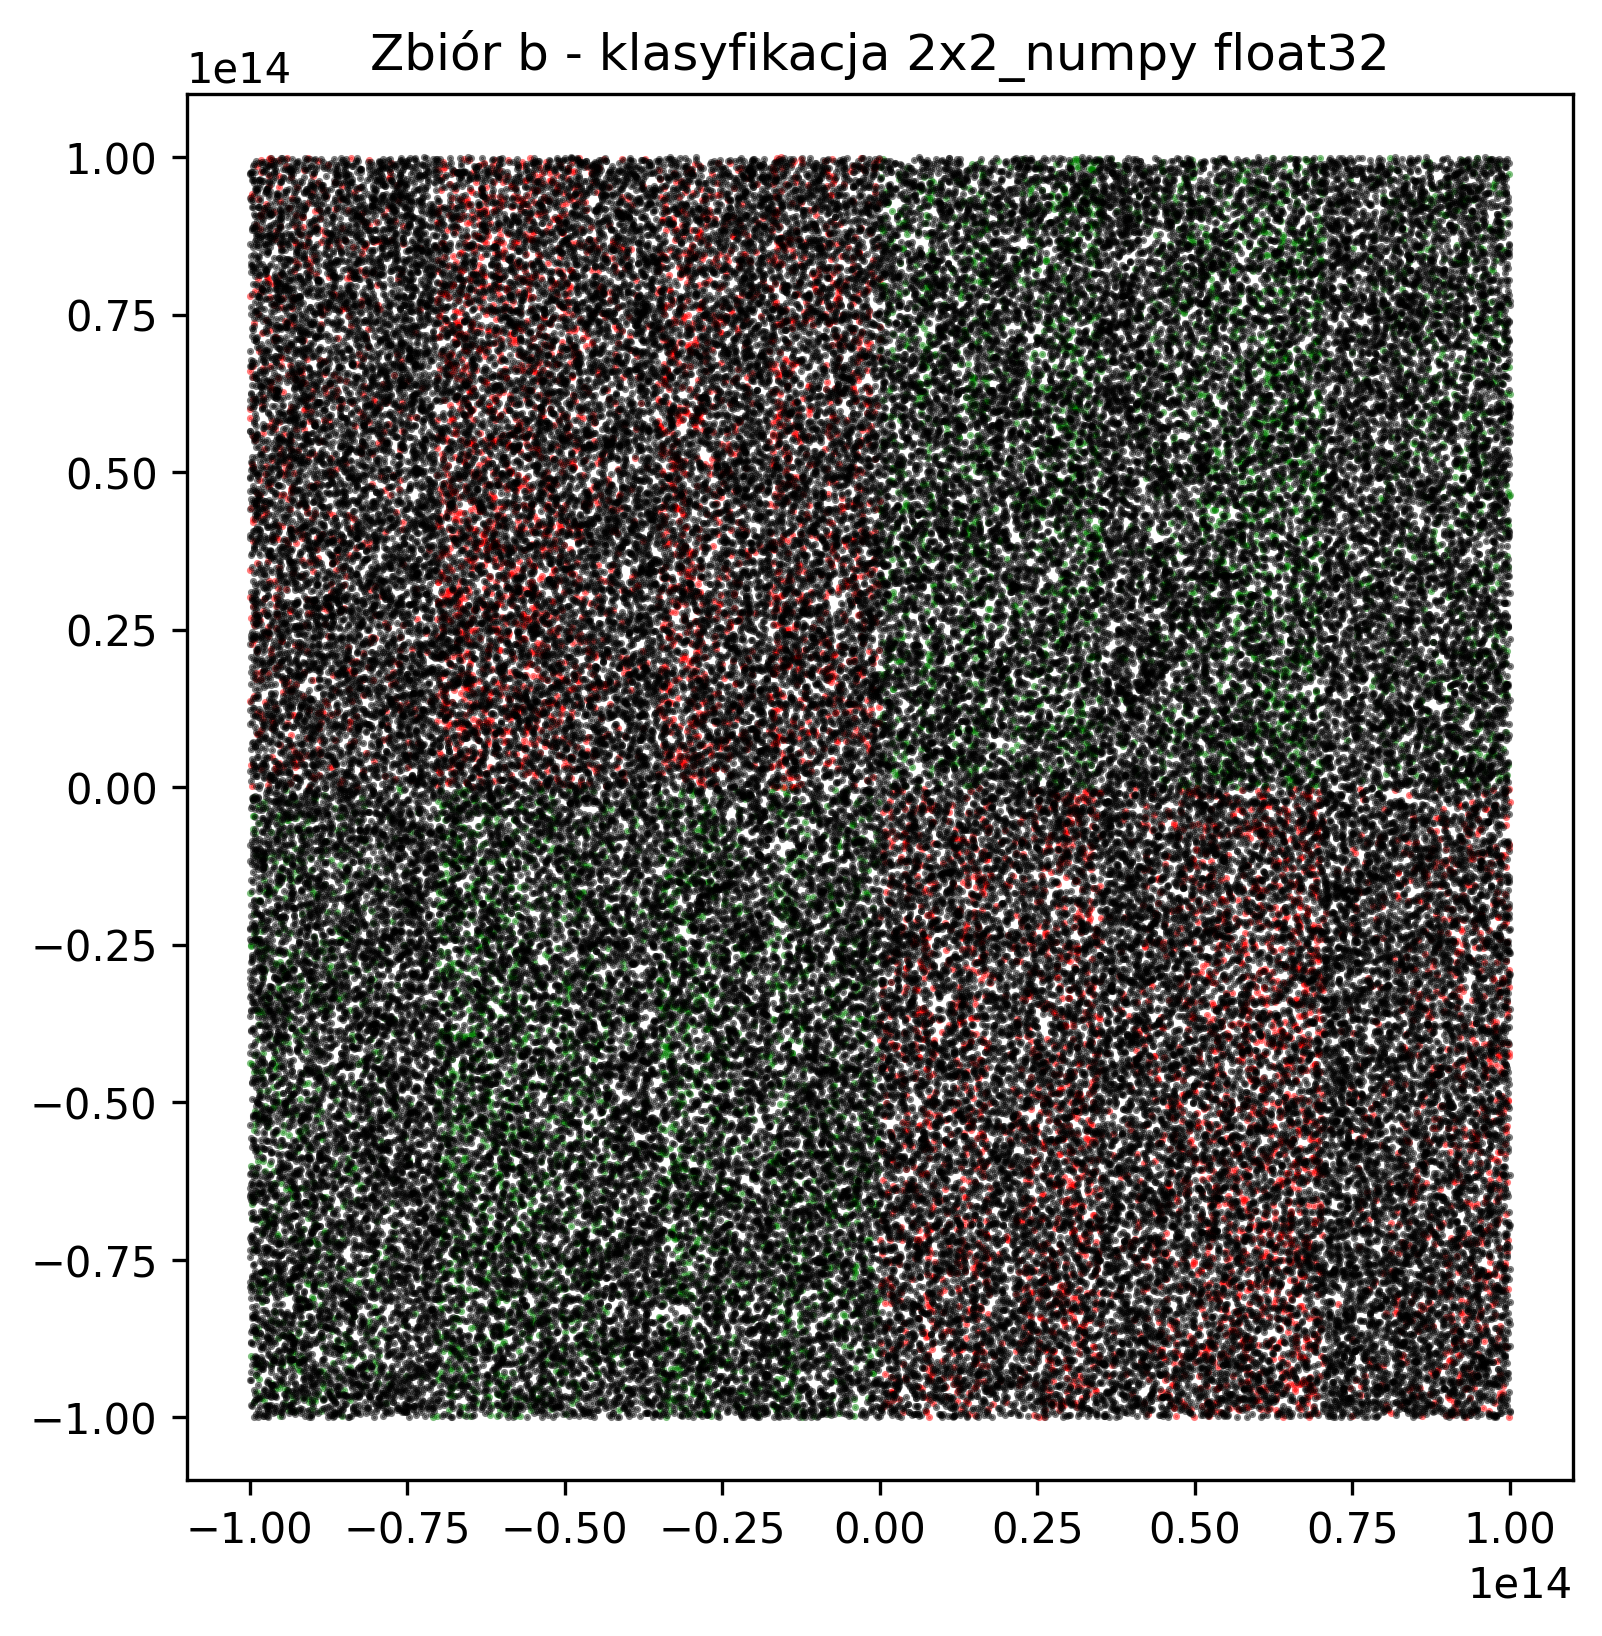
\includegraphics[width=\linewidth]{plots/dataset_Zbiór b - klasyfikacja 2x2_numpy float32_1e-06.png}
        \caption{Klasyfikacja punktów ze zbioru b metodą \texttt{2x2\_numpy} na typie \texttt{float32}.}
        \label{fig:classified_b_32}
    \end{minipage}
\end{figure}

\begin{table}[htbp]
    \centering
    \caption{Zestawienie wyników klasyfikacji dla zbioru b.}
    \label{tab:wyniki_b_all_eps}
    \begin{tabular}{llllllll}
        \toprule
        Zbiór & Typ danych & Epsilon & Metoda & Czas [s] & Lewa & Prawa & Współliniowe \\
        b & \texttt{float64} & $10^{-12}$ & \texttt{3x3}        & 0.0063 & 50042 & 49958 & 0 \\
        b & \texttt{float64} & $10^{-12}$ & \texttt{3x3\_numpy} & 0.0273 & 50042 & 49958 & 0 \\
        \midrule
        b & \texttt{float32} & $10^{-12}$ & \texttt{3x3}        & 0.0026 & 50042 & 49958 & 0 \\
        b & \texttt{float32} & $10^{-12}$ & \texttt{3x3\_numpy} & 0.0346 & 50042 & 49958 & 0 \\
        \midrule
        b & \texttt{float64} & $10^{-12}$ & \texttt{2x2}        & 0.0032 & 50037 & 49951 & 12 \\
        b & \texttt{float64} & $10^{-12}$ & \texttt{2x2\_numpy} & 0.0189 & 50036 & 49950 & 14 \\
        \midrule
        b & \texttt{float32} & $10^{-12}$ & \texttt{2x2}        & 0.0018 & 0     & 0     & 100000 \\
        b & \texttt{float32} & $10^{-12}$ & \texttt{2x2\_numpy} & 0.0157 & 6623  & 6618  & 86759 \\
        \bottomrule
    \end{tabular}
\end{table}

\subsection{Zbiór d}

Wyniki klasyfikacji w zbiorze d okazały się najbardziej czułe na wybór wartości $\epsilon$, typu danych oraz metody liczenia wyznacznika. 
Tak samo jak w zbiorze b, typ \texttt{float32} powodował bardzo duże błędy w obliczeniach z powodu zbyt niskiej precyzji.

Wszystkie punkty poprawnie zakwalifikowały tylko metody używające wyznacznika macierzy $3 \times 3$ na typie \texttt{float64}. 

Dla wszystkich pozostałych metod zmniejszanie tolerancji dla zera powodowało zwiększanie ilości źle sklasyfikowanych punktów.

Na Rysunkach \ref{fig:classified_d_3x3_64}, \ref{fig:classified_d_3x3_32}, \ref{fig:classified_d_2x2_64} i \ref{fig:classified_d_2x2_32} porównano klasyfikacje punktów na prostej używając wyznaczników macierzy $2 \times 2$ i $3 \times 3$ oraz typów danych \texttt{float32} i \texttt{float64}.

W Tabeli \ref{tab:wyniki_d_all} przedstawiono wyniki dla wszystkich metod, typów danych i epsilonów.

\begin{figure}[htbp]
    \centering
    \begin{minipage}{0.48\textwidth}
        \centering
        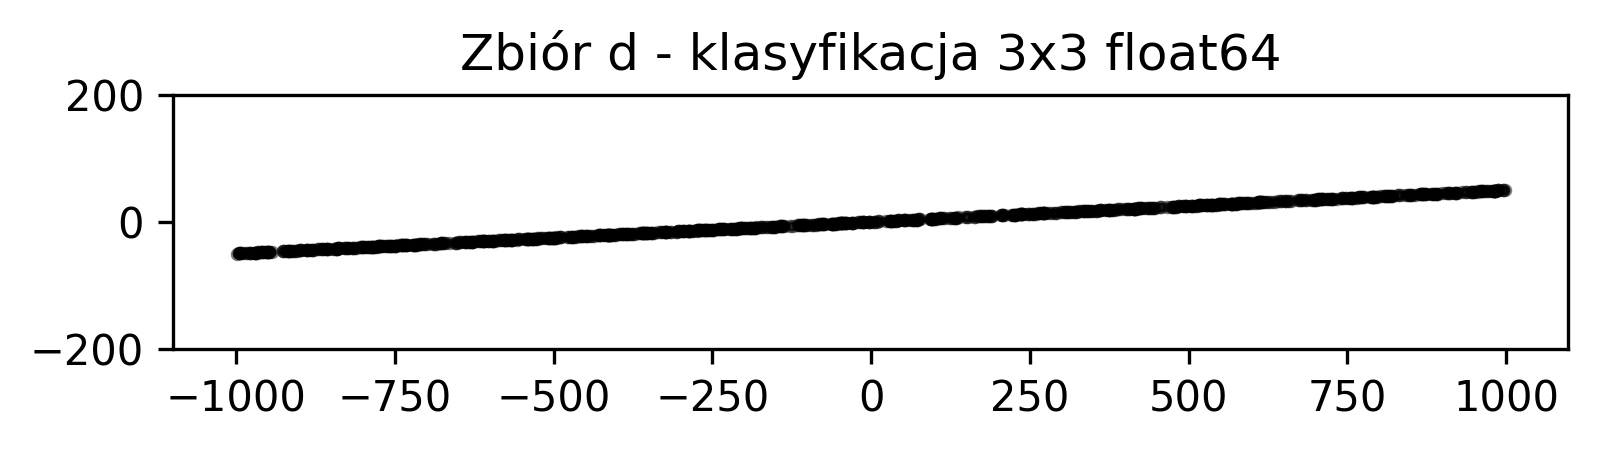
\includegraphics[width=\linewidth]{plots/dataset_Zbiór d - klasyfikacja 3x3 float64_1e-12.png}
        \caption{Klasyfikacja punktów ze zbioru d metodą \texttt{3x3} na typie \texttt{float64}.}
        \label{fig:classified_d_3x3_64}
    \end{minipage}
    \hfill
    \begin{minipage}{0.48\textwidth}
        \centering
        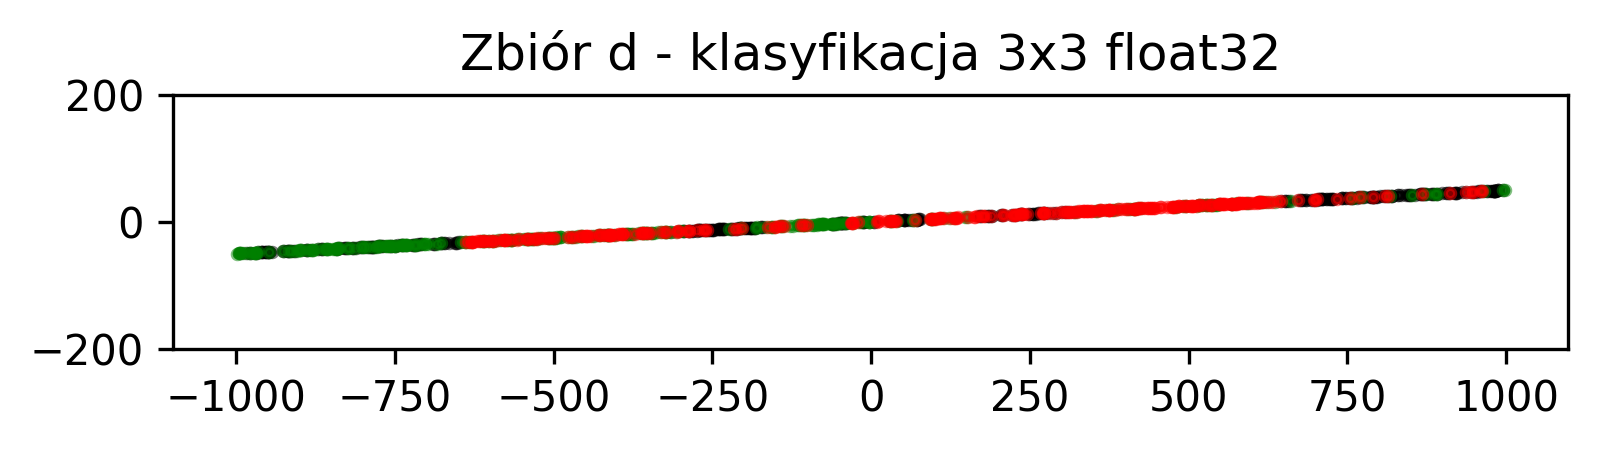
\includegraphics[width=\linewidth]{plots/dataset_Zbiór d - klasyfikacja 3x3 float32_1e-12.png}
        \caption{Klasyfikacja punktów ze zbioru d metodą \texttt{3x3} na typie \texttt{float32}.}
        \label{fig:classified_d_3x3_32}
    \end{minipage}
\end{figure}

\begin{figure}[htbp]
    \centering
    \begin{minipage}{0.48\textwidth}
        \centering
        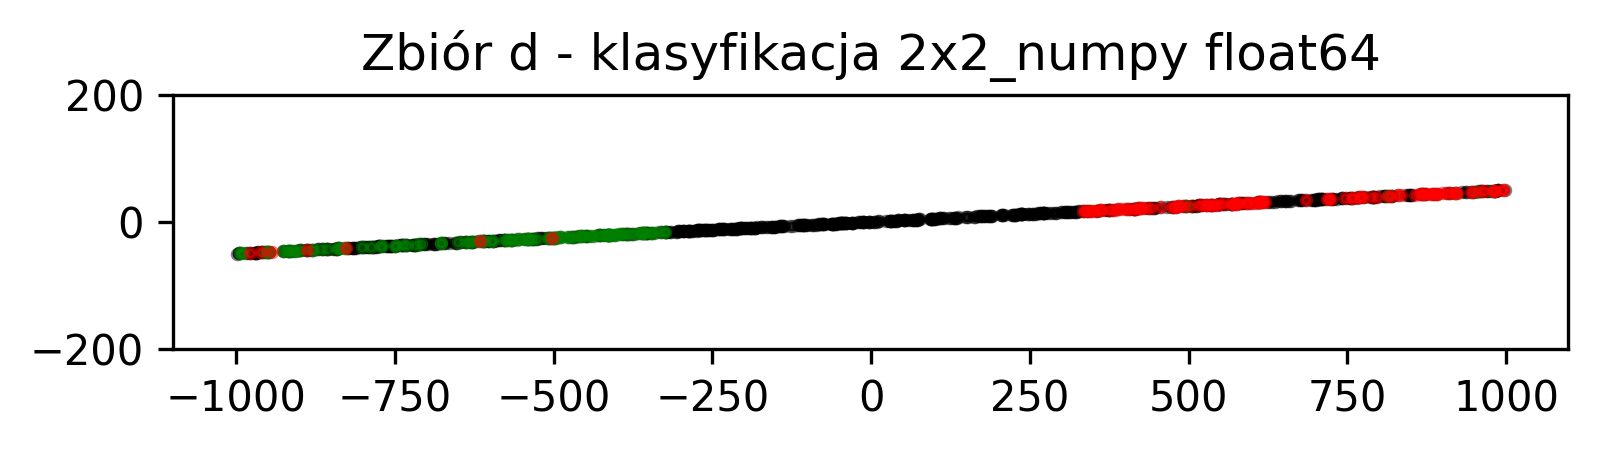
\includegraphics[width=\linewidth]{plots/dataset_Zbiór d - klasyfikacja 2x2_numpy float64_1e-12.png}
        \caption{Klasyfikacja punktów ze zbioru d metodą \texttt{2x2\_numpy} na typie \texttt{float64}.}
        \label{fig:classified_d_2x2_64}
    \end{minipage}
    \hfill
    \begin{minipage}{0.48\textwidth}
        \centering
        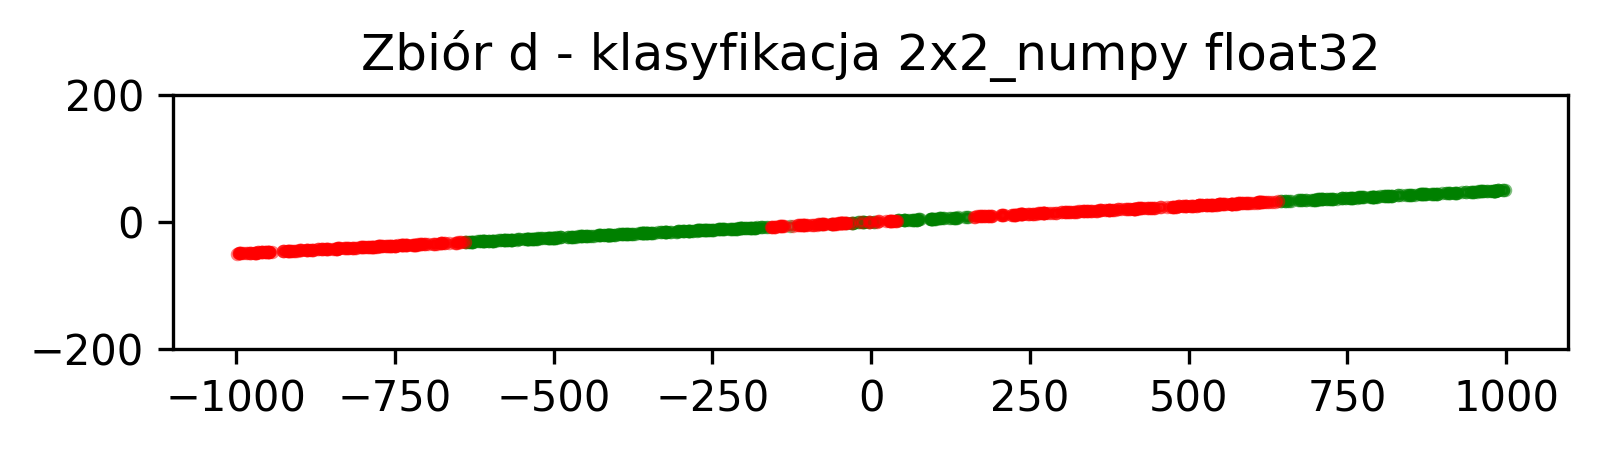
\includegraphics[width=\linewidth]{plots/dataset_Zbiór d - klasyfikacja 2x2_numpy float32_1e-12.png}
        \caption{Klasyfikacja punktów ze zbioru d metodą \texttt{2x2\_numpy} na typie \texttt{float32}.}
        \label{fig:classified_d_2x2_32}
    \end{minipage}
\end{figure}

\begin{table}[htbp]
    \centering
    \caption{Zestawienie wyników klasyfikacji dla zbioru d.}
    \label{tab:wyniki_d_all}
    \begin{tabular}{llllllll}
        \toprule
        Zbiór & Typ danych & Epsilon & Metoda & Czas [s] & Lewa & Prawa & Współliniowe \\
        \midrule
        d & \texttt{float64} & $10^{-6}$  & \texttt{3x3}        & 0.0001 & 0   & 0   & 1000 \\
        d & \texttt{float64} & $10^{-9}$  & \texttt{3x3}        & 0.0001 & 0   & 0   & 1000 \\
        d & \texttt{float64} & $10^{-12}$ & \texttt{3x3}        & 0.0001 & 0   & 0   & 1000 \\
        \midrule
        d & \texttt{float64} & $10^{-6}$  & \texttt{2x2}        & 0.0000 & 0   & 0   & 1000 \\
        d & \texttt{float64} & $10^{-9}$  & \texttt{2x2}        & 0.0000 & 0   & 0   & 1000 \\
        d & \texttt{float64} & $10^{-12}$ & \texttt{2x2}        & 0.0001 & 94  & 67  & 839  \\
        \midrule
        d & \texttt{float64} & $10^{-6}$  & \texttt{3x3\_numpy} & 0.0003 & 0   & 0   & 1000 \\
        d & \texttt{float64} & $10^{-9}$  & \texttt{3x3\_numpy} & 0.0003 & 0   & 0   & 1000 \\
        d & \texttt{float64} & $10^{-12}$ & \texttt{3x3\_numpy} & 0.0003 & 0   & 0   & 1000 \\
        \midrule
        d & \texttt{float64} & $10^{-6}$  & \texttt{2x2\_numpy} & 0.0002 & 0   & 0   & 1000 \\
        d & \texttt{float64} & $10^{-9}$  & \texttt{2x2\_numpy} & 0.0002 & 0   & 0   & 1000 \\
        d & \texttt{float64} & $10^{-12}$ & \texttt{2x2\_numpy} & 0.0002 & 118 & 110 & 772  \\
        \midrule
        d & \texttt{float32} & $10^{-6}$  & \texttt{3x3}        & 0.0001 & 253 & 261 & 486  \\
        d & \texttt{float32} & $10^{-9}$  & \texttt{3x3}        & 0.0000 & 314 & 304 & 382  \\
        d & \texttt{float32} & $10^{-12}$ & \texttt{3x3}        & 0.0000 & 314 & 304 & 382  \\
        \midrule
        d & \texttt{float32} & $10^{-6}$  & \texttt{2x2}        & 0.0000 & 152 & 148 & 700  \\
        d & \texttt{float32} & $10^{-9}$  & \texttt{2x2}        & 0.0001 & 156 & 150 & 694  \\
        d & \texttt{float32} & $10^{-12}$ & \texttt{2x2}        & 0.0000 & 156 & 150 & 694  \\
        \midrule
        d & \texttt{float32} & $10^{-6}$  & \texttt{3x3\_numpy} & 0.0003 & 249 & 254 & 497  \\
        d & \texttt{float32} & $10^{-9}$  & \texttt{3x3\_numpy} & 0.0003 & 407 & 410 & 183  \\
        d & \texttt{float32} & $10^{-12}$ & \texttt{3x3\_numpy} & 0.0003 & 407 & 410 & 183  \\
        \midrule
        d & \texttt{float32} & $10^{-6}$  & \texttt{2x2\_numpy} & 0.0003 & 487 & 483 & 30   \\
        d & \texttt{float32} & $10^{-9}$  & \texttt{2x2\_numpy} & 0.0002 & 502 & 497 & 1    \\
        d & \texttt{float32} & $10^{-12}$ & \texttt{2x2\_numpy} & 0.0002 & 502 & 498 & 0    \\
        \bottomrule
    \end{tabular}
\end{table}

\section{Wnioski}

Przeprowadzone eksperymenty można podsumować w następujących punktach:

\begin{enumerate}
    \item \textbf{Wybór precyzji zmiennoprzecinkowej:} 
    Wybór typu danych miał największy wpływ na poprawność wyników. Typ \texttt{float32} charakteryzujący się mniejszą precyzją niż \texttt{float64} prowadził do dużo większych błędów zaokrągleń i fałszywych klasyfikacji.
    
    \item \textbf{Wpływ wielkości danych:} W zbiorze b, przy współrzędnych rzędu $10^{14}$ zastosowanie typu \texttt{float32} skutkowało drastyczną utratą cyfr znaczących w wyniku odejmowania bliskich sobie liczb, co doprowadziło do sytuacji, w której algorytm $2 \times 2$ błędnie zakwalifikował 100\% punktów jako współliniowe. W zbiorach a i c, gdzie współrzędne były wielkości tylko $10^3$ i $10^2$ wszystkie metody działały całkowicie poprawnie.

    \item \textbf{Metoda liczenia wyznacznika:} Metoda oparta na wyznaczniku stopnia 3 ($3 \times 3$) okazała się znacznie stabilniejsza numerycznie niż metoda $2 \times 2$ , która wykazała dużo większą wrażliwość na błędy zaokrągleń.
    
    \item \textbf{Wpływ progu tolerancji ($\epsilon$):} 
    Im niższa tolerancja dla zera tym na mniejszy margines błędu pozwalamy. Przez ograniczoną precyzję reprezentacji liczb w komputerze jednak wybranie zbyt restrykcyjnego progu powoduje utratę poprawności, co widać najlepiej przy zbiorze d (wszystkie punkty na prostej).
    
    
    \item \textbf{Wydajność metod własnych oraz bibliotecznych:}
    Metody z biblioteki NumPy w niektórych zbiorach były dokładniejsze niż metody własne, a w innych mniej dokładne. W każdym zbiorze jednak metody własne były szybsze od tych bibliotecznych.
    
\end{enumerate}

\end{document}
